\section{Examples}
In this section we describe in detail some worked out examples and
give the corresponding code. All examples can also be found in the
{\texttt{examples}} subdirectory of \mpspack.

\subsection{Acoustic scattering from the unit square}

\subsubsection{Problem description and solution approach}

In this example we solve the problem of time-harmonic 
acoustic sound-soft scattering from the unit square $\Omega=(-0.5,0.5)^2$.
The full PDE has the following form.
\begin{eqnarray}
\Delta u+k^2u & = & 0  \quad \text{in
}\mathbb{R}^2\backslash\Omega\label{eq:helm}\\
u&=&0 \quad \text{on } \pO \label{eq:soundsoft}\\
\frac{\partial u_s}{\partial r}-iku_s & = & o(r^{-1/2}),\label{eq:sommerfeld}
\end{eqnarray}
Here, $u=u_{inc}+u_s$ is the total field, $u_{inc}$ is the incident
wave, $u_s$ is the scattered field, and $r$ is the radial coordinate.
The Sommerfeld radiation condition
\eqref{eq:sommerfeld} is to be understood to hold uniformly in all
directions. 

\begin{figure}
\center
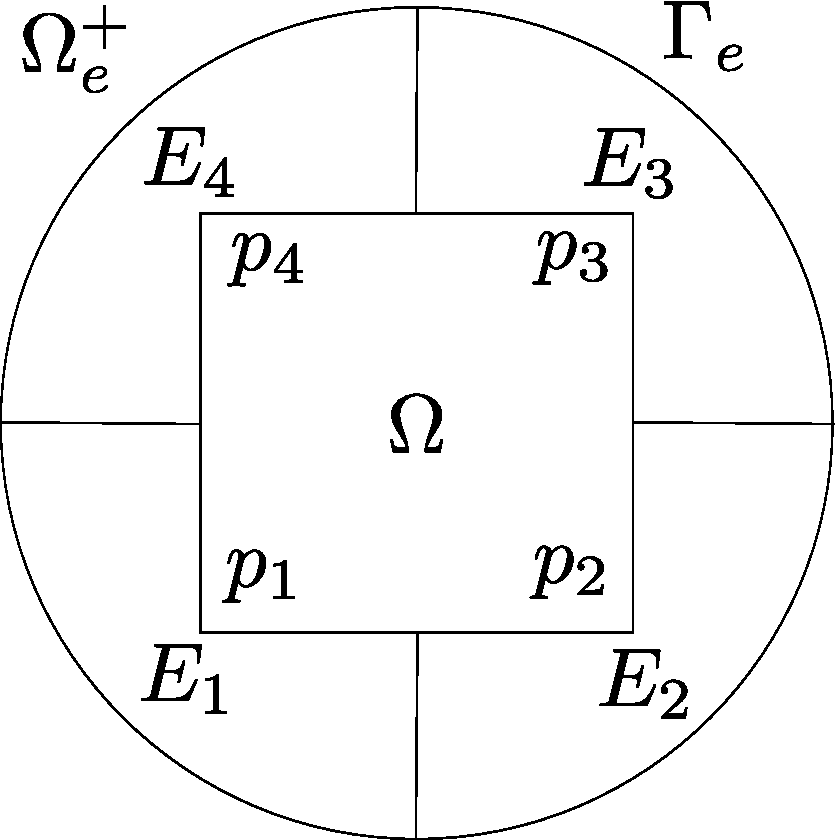
\includegraphics[width=6cm]{geometry}
\vspace{-.5cm}
\label{fig:geom}
\end{figure}


To achieve high accuracy we cannot simply use fundamental soluitions
to approximate the scattered field. The problem is the singularities
of the solution $u$ at the corners. If these are not represented in
the basis our approximation error will decay very slowly as the number
of basis functions increases. To solve this problem we use the domain
decompositon shown in Figure \ref{fig:geom}. The idea is that each of
the elements $E_i$ only contains one corner $p_i$ of the square. We can then
match the corner behavior in each domain by using fractional order
Bessel functions. Since furthermore, $u=0$ on $\partial\Omega$ it will
be sufficient to use Fourier-Bessel sine functions that automatically
satisfy the zero boundary conditions on the sides of the square.
Hence, the total field $u$ is approximated in each element $E_i$ using
an approximation of the form
$$
u(r,\theta)\approx
\sum_{j=1}^{N_i}c_j^{(i)}J_{\frac{2}{3}j}(kr)\sin(\frac{2j}{3}\theta).
$$
The polar coordinate system in each element $E_i$ is rotated in such a way
that the basis functions are zero on the sides adjacent to the corner
at $p_i$.

In the infinite domain $\Omega_e^+$ we use a basis of fundamental
solutions to represent the scattered field $u_s$. Hence, for
$\bx\in\Omega^+$ we have
$$
u_s(\bx)\approx \sum_{j=1}^{N_e}\frac{i}{4}c_j^{(e)}H_0^{(1)}(|\bx-\by_j|),
$$
where $\by_j=r_{mfs}e^{i\phi_j}$ and $\phi_j=\frac{2\pi j}{N_e}$. Note
that we approximate with the fundamental solutions the scattered field
$u_s$ while in the finite subdomains $E_i$ we approximate the total
field $u$. The compatibility conditions between approximations $u^{i}$
und $u^{j}$ in two neighboring elements $E_i$ and $E_j$ with common
boundary $\Gamma_{ij}$ are given by
$$
u^{(i)}(\bx)\approx u^{(j)}(\bx),\quad \frac{\partial u}{\partial
  n_i}{u^{(i)}}(\bx)\approx  \frac{\partial u}{\partial
  n_i}{u^{(j)}}(\bx),
$$
where $\bx\in\Gamma_{ij}$ and $\frac{\partial}{\partial\nu_i}$ is the
outward normal derivative at the boundary of $E_i$.
On the interface $\Gamma_{ie}$ between an element $E_i$ and the
exterior domain $\Omega_e^{+}$ we have the compatibility conditions
$$
u^{(i)}(\bx)\approx u_{inc}(\bx)+u_s^{(e)}(\bx),\quad \frac{\partial}{\partial
  n_i}{u^{(i)}}(\bx)\approx  \frac{\partial}{\partial
  n_i}{(u_s^{(e)}+u_{inc})}(\bx),
$$
where $u_s^{(i)}$ is the fundamental solutions approximation to the
scattered field in $\Omega_e^{+}$. We have to add the incident field
to the approximate scattered field since we are matching with the
total field in the elements $E_i$.
An approximate solution to the whole problem is now 
computed by minimizing the $L^2$ error of 
the compatibility conditions on all interfaces.

\subsubsection{Implementation in \mpspack}

Although the setup of the problem seems quite complicated we will see
that it is very simple to set it up in \mpspack. Indeed, the most part
of the code will be devoted to creating the mesh structure from
Figure \ref{fig:geom}.

\paragraph{Initialization of the problem parameters}

We need to define the following problem parameters.
\begin{verbatim}
k = 50;      % Wavenumber
r = 1.0;     % Radius of outer circle    
M = 200;     % Number of quadrature points on segments
N=100;       % Number of basis fct. in each subdomain
a=.5;        % Half-Size of the square
rmfs=0.8*r;  % Radius of the fundamental solutions curve
\end{verbatim}


\paragraph{Setup of the geometry}

We now need to define the geometry. Fortunately,
\mpspack gives some support for the construction of the geometry.

First we define the segments of one element ($E_3$ in Figure
\ref{fig:geom}). This is done with the following three commands.

\begin{verbatim}
s = segment.polyseglist(M, [1i*r 1i*a a+1i*a a r], 'g');
s=[s(1:3) segment(2*M, [0 r 0 pi/2])];
s = [s rotate(s, pi/2) rotate(s, pi) rotate(s, 3*pi/2)];
\end{verbatim}
The first command defines all the straight lines that form part of the
boundary of $E_3$. For this we use {\texttt{polyseglist}}. The command
{\texttt polyseglist} constructs a closed polygon. We then delete the
last two segments of the array {\texttt s} and add instead the
circular line segment. This results in the segments shown in the left
plot of Figure \ref{fig:elem1}. We now rotate this element three times to
obtain the segments showin in the right plot of Figure \ref{fig:circelem}.
\begin{figure}
\begin{tabular}{cc}
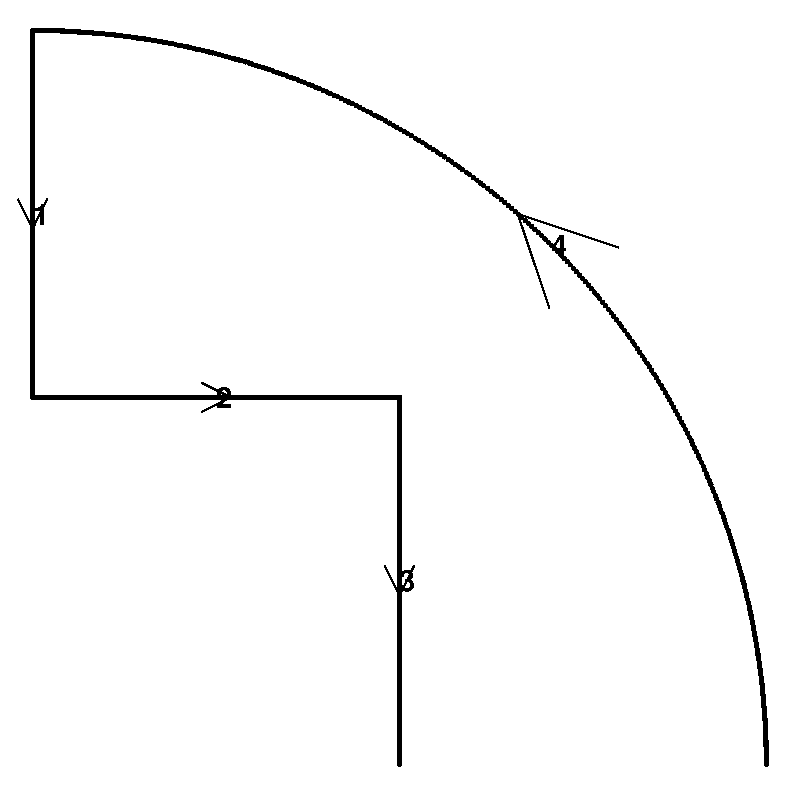
\includegraphics[width=5cm]{circelem1} &
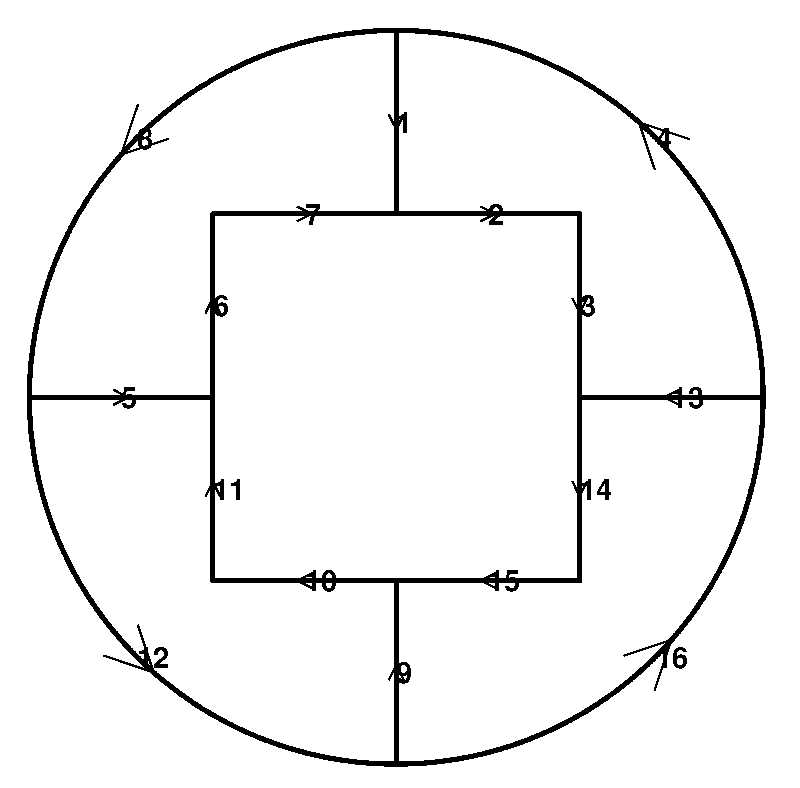
\includegraphics[width=5cm]{circelem2}
\end{tabular}
\caption{The segments in the right plot are created by rotating the segments
  shown in the left plot.}
\label{fig:circelem}
\end{figure}

For later it is important to have a separate list of all segments not
belonging to the square and all segments belonging to the outer
circle.

\begin{verbatim}
sdecomp=s([1 4 5 8 9 12 13 16]); % All artificial boundaries
extlist=s([4 8 12 16]);          % Segments forming the outer circle
\end{verbatim}

We now define the domains. By taking the rotational symmetry into
account we can do this in a simple for loop.

\begin{verbatim}
d=domain.empty(4,0);
for j=1:4, d(j)=domain(s(1+mod(4*(j-1)+[0 1 2 12 3],16)),[1 1 1 -1 1]); end
ext = domain([], [],extlist(end:-1:1), -1); 
\end{verbatim}
The for loop looks slightly complicated. But all it does is pick out
the right indices for the elements forming a domain and creating it
together with the right sense of direction. At the end we have an
array {\texttt d} containing the four fine domains $E_i$. The exterior
domain {\texttt ext} is created by traversing {\texttt extlist} in
reverse order with reversed sense $-1$. This is necessary since we now
have the boundary of an exterior domain, which has a reversed sense of
direction.

Setting up the compatibility conditions is now trivial. It is done by
the command
\begin{verbatim}
sdecomp.setmatch([k -k],[1 -1]);
\end{verbatim}
The matching conditions for the function values are scaled by the
wavenumber $k$ to balance the different scaling between the $L^2$ error
in the function and the $L^2$ error in the
derivative.\footnote{Consider the one dimensional plane wave
  $e^{ikx}$. The derivative is $ike^{ikx}$. Hence, in general it makes sense to
  scale the $L^2$ error of function values by $k$ to give it the same
  dimension as the $L^2$ error of the derivative.}

We can now add the basis functions to the domains. The fractional
Bessel functions are added to the interior domains by the following
command.
\begin{verbatim}
nuopts=struct('type','s','cornermultipliers',[0 0 1 0 0],'rescale_rad',1);
for j=1:4, d(j).addcornerbases(N,nuopts); end
\end{verbatim}
The options structure {\texttt nuoopts} specifies that we only want
Fourier-Bessel sine functions at the third corner of each domain. This
is the corner belonging to the square. The option {\texttt
  'rescale\_rad'} specifies that the basis functions are rescaled to
balance out the bad scaling of Bessel functions. The method {\texttt
  addcornerbases} automatically finds out the right fractional orders,
offsets and suitable branch vectors.

The exterior fundamental solutions are added with the following command.
\begin{verbatim}
Z=@(t) rmfs*exp(2i*pi*t); Zp=@(t) 2i*pi*rmfs*exp(2i*pi*t);
opts=struct('eta','k','fast',1,'nmultiplier',2);
ext.addmfsbasis({Z, Zp},N,opts);
\end{verbatim}
Note that now {\texttt nmultiplier} is set to $2$. It turns out to be
effective for this problem to use twice as many fundamental solutions
as there are Fourier-Bessel sine functions in each domain.

We now have everything together to setup the problem class and solve
the scattering problem. The following commands setup the scattering
problem and define an incident plane wave.
\begin{verbatim}
pr=scattering(ext,d);
pr.setoverallwavenumber(k);
pr.setincidentwave(-pi/4);
\end{verbatim}
There is one small specialty here. In the first line we have 
defined {\texttt ext} to be an air-domain and the array {\texttt d} to
be a non-air domain. This tells \mpspack~to add the incident field to
the exterior basis functions in assembling the least-squares problem.

The following commands now solve the problem and plot the solution
$u$.
\begin{verbatim}
tic; pr.solvecoeffs; fprintf('\tcoeffs done in %.2g sec\n', toc)
fprintf('\tL2 bdry error norm = %g, coeff norm = %g\n', ...
        pr.bcresidualnorm, norm(pr.co))
o.bb=[-1.5 1.5 -1.5 1.5];
o.dx=0.02;

[ui gx gy] = pr.gridincidentwave(o);
u = pr.gridsolution(o);

figure;
imagesc(gx, gy, real(ui+u)); title('Full Field (Real Part)');
c = caxis; caxis([-1 1]*max(c));
axis equal tight;
colorbar;
set(gca,'ydir','normal'); 
\end{verbatim}
The incident field {\texttt ui} 
is automatically evaluated only in air-domains. If
we want to evaluate it in all domains we have to set {\texttt
  o.all=1}. But here the default behavior is fine for us. The sum
{\texttt ui+u} is now the total field in all domains (remember that
{\texttt u} approximates the total field in the interior domains
and the scattered field in the exterior domain). The {\texttt
  scattering} class also provides a routine {\texttt showthreefields}
to plot the incident wave, scattered field and total field. However,
the routine assumes that the computed solution is the scattered field,
which is not correct for the way we have set up this problem.

The output of the example problem is shown in Figure \ref{fig:squareplot}.
\begin{figure}
\center
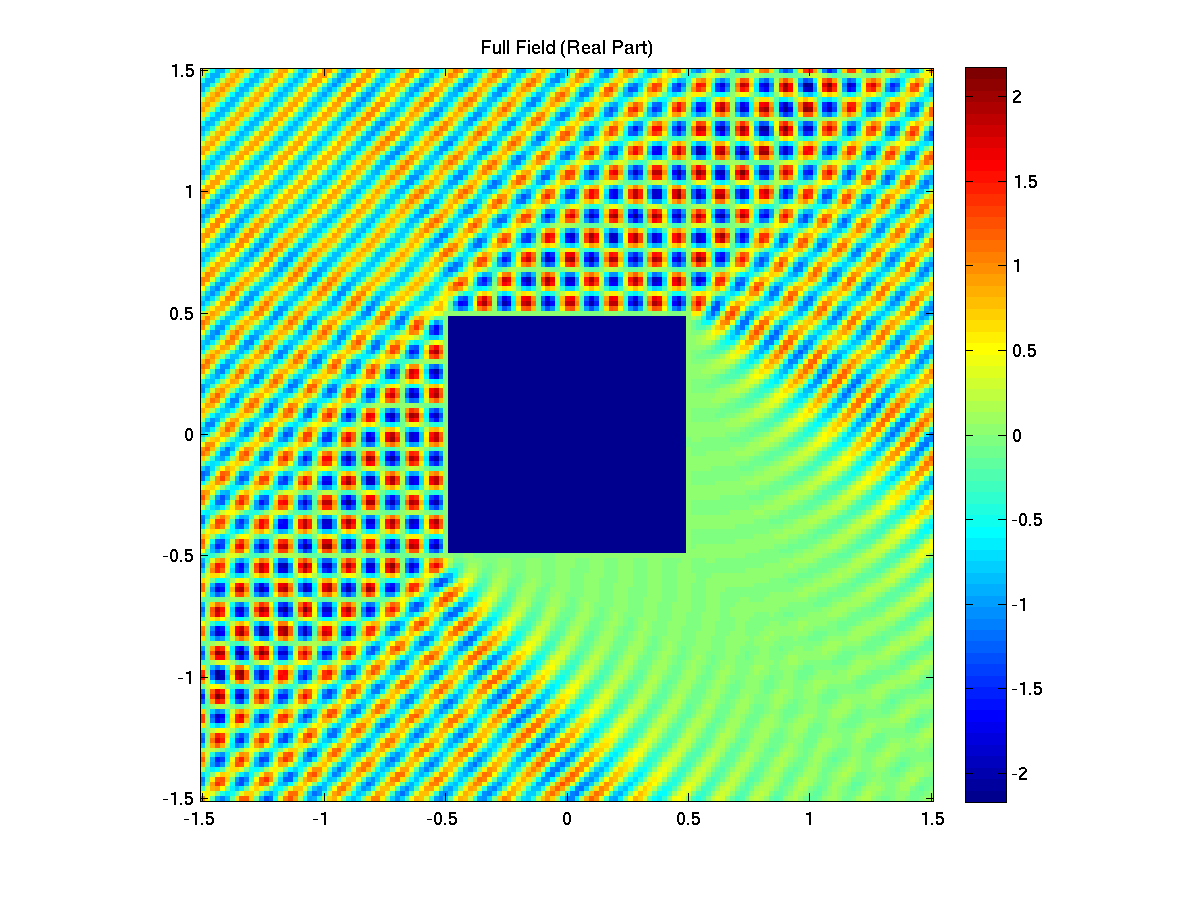
\includegraphics[width=8cm]{squareplot}
\caption{The solution of the scattering problem on the unit
  square with sound-soft boundary conditions.}
\label{fig:squareplot}
\end{figure}
The $L^2$ boundary error of the solution is approximately $1.5\cdot
10^{-10}$. On a standard laptop with Intel Core 2 Duo processor the
solution vector is computed in around $11$ seconds. The plot takes
slightly longer.

A wonderful feature of this approach is that we can trivially switch
to a sound-hard scattering problem, that is instead of requiring $u=0$
on $\partial\Omega$ we require $\frac{\partial}{\partial n} u=0$ on
$\partial\Omega$. All we have to do is switch to Fourier-Bessel cosine
functions. These automatically satisfy the required condition for the
normal derivative. The solution to this problem is shown in Figure
\ref{fig:squareplot2}.
\begin{figure}
\center
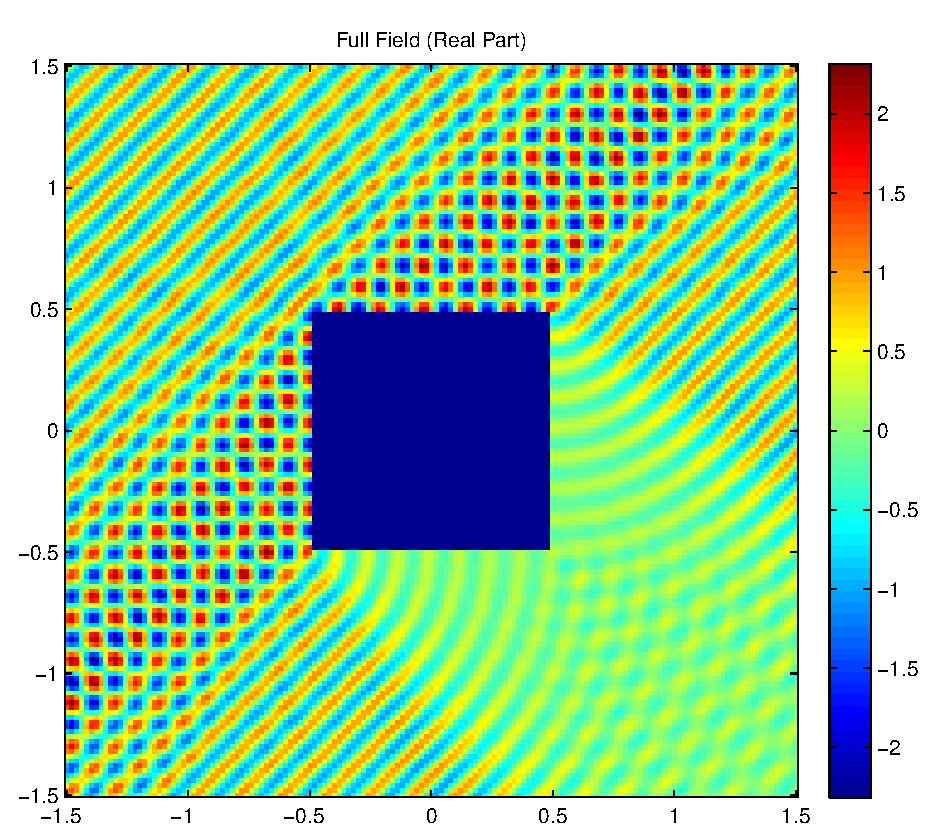
\includegraphics[width=8cm]{squareplot2}
\caption{The solution of the scattering problem on the unit
  square with sound-hard boundary conditions.}
\label{fig:squareplot2}
\end{figure}
The accuracy and solution time are comparable to the sound-soft
scattering place.

%%% Local Variables: 
%%% mode: latex
%%% TeX-master: "tutorial"
%%% End: 
